\documentclass[a4paper,10pt]{article}
%\documentclass[a4paper,10pt]{scrartcl}

\usepackage[utf8]{inputenc}
\usepackage[german]{babel}
\usepackage[pdftex]{graphicx}
\usepackage{listings}
\usepackage{color}
\usepackage{amssymb}
\usepackage{marvosym}
\usepackage{amsmath}
\usepackage{array}
\usepackage{geometry}
\usepackage{listings}
\usepackage{upgreek}
\usepackage{color}
\usepackage{gensymb}

\geometry{verbose,tmargin=2cm,bmargin=2cm,lmargin=2cm,rmargin=2.5cm,headheight=80pt}

\newcommand{\f}{\textbf}

\title{Formeln SSD}
\author{}
\date{}


\pdfinfo{%
  /Title    ()
  /Author   ()
  /Creator  ()
  /Producer ()
  /Subject  ()
  /Keywords ()
}

\begin{document}
\maketitle

\section*{Bahn- und Orbitdinge}
\f{3. Keplersches Gesetz} (Quadrate der Umlaufdauern proportional zu den Kuben der großen Halbachsen)
\[T = 2\pi\sqrt{\frac{a^3}{\mu}}\]
\f{Ellipsendinge}:
\begin{figure}[!ht]
 \centering
 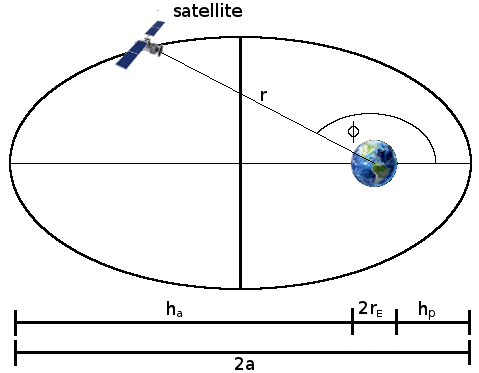
\includegraphics[scale=0.5]{pic1.png}
\end{figure}
\[2a = h_a + h_p + 2r_E\]
\[r_p = h_p + r_E \text{\qquad \qquad} r_a = h_a + r_E\]
\[r_p = a(1-\varepsilon) \text{\qquad \qquad} r_a = a(1+\varepsilon)\]
\[\varepsilon = \frac{r_p - r_a}{r_p + r_a}\]
\f{Vis-Viva-Gleichung/Binet-Gleichung}:
\[v = \sqrt{\mu\left(\frac{2}{r} -\frac{1}{a}\right)}\]
\f{Vis-Viva-Gleichung für Kreis}:
\[r = a \Rightarrow v = \sqrt{\frac{\mu}{r}} \]
für Erde: 
\[v = \sqrt{\frac{\mu}{r_E}} = 7.905 \frac{km}{s}\]
(= erste kosmische Geschwindigkeit = minimale Geschwindigkeit, die ein Objekt haben muss, um in einen Erdorbit zu gelangen) \\
\vspace*{5pt}

\noindent \f{Vis-Viva-Gleichung für Parabel}:
\[a \rightarrow \infty \Rightarrow v = \sqrt{\frac{2\mu}{r}} \]
für Erde: 
\[v = \sqrt{\frac{2\mu}{r_E}} = 11.179 \frac{km}{s}\]
(= zweite kosmische Geschwindigkeit = minimale Geschwindigkeit, die ein Objekt haben muss, um das Gravitationsfeld der Erde zu verlassen) \\
\vspace*{5pt}

\noindent \f{Geschwindigkeitsdinge für Ellipse}:\\
\vspace*{3pt}

\noindent average angular velocity:
\[ \frac{2\pi}{T} \frac{\text{rad}}{\text{min}} ~~~ \frac{360\degree}{T} \frac{\text{deg}}{\text{min}}\]
maximale Geschwindigkeit (Periapsis):
\[v_{max} = \sqrt{\mu\left(\frac{2}{h_p+r} -\frac{1}{a}\right)}\]
minimale Geschwindigkeit (Apoapsis):
\[v_{min} = \sqrt{\mu\left(\frac{2}{h_a+r} -\frac{1}{a}\right)}\]
wahre Anomalie ($\Phi$, $\nu$, ...)
\[r = a\frac{1-\varepsilon^2}{r\cdot \varepsilon \cdot cos(\nu)} \Rightarrow \nu = arccos\left(a\frac{1-\varepsilon^2}{r^2\cdot \varepsilon}\right)\]
wahre Anomalie ist auch über die exzentrische Anomalie berechenbar:
\[tan\left(\frac{\nu}{2}\right) = \sqrt{\frac{1+\varepsilon}{1-\varepsilon}}\cdot tan\left(\frac{E}{2}\right)\]
\[E - \varepsilon \cdot sin(E) = \frac{2\pi}{T}(t-t_{perigee})\]
right ascension of the ascending node:
\[\Delta \Omega_{rev} = -\frac{3\pi J_2r_E^2}{a^2(1-\varepsilon^2)^2}cos(i) \text{\qquad  in} \left[\frac{\text{rad}}{\text{rev}}\right]\]
\[\Delta \Omega_{rev} = -\frac{3\pi J_2r_E^2}{a^2(1-\varepsilon^2)^2}cos(i) \cdot \frac{360^{\circ}}{2\pi} \text{\qquad  in} \left[\frac{\text{deg}}{\text{rev}}\right]\]
\[\Delta \Omega_{day} = -\frac{3\pi J_2r_E^2}{a^2(1-\varepsilon^2)^2}cos(i) \cdot \frac{\uptau_E}{T} \text{\qquad  in} \left[\frac{\text{rad}}{\text{day}}\right]\]
\[\Delta \Omega_{rev} = -\frac{3\pi J_2r_E^2}{a^2(1-\varepsilon^2)^2}cos(i) \cdot \frac{360^{\circ}}{2\pi}\cdot \frac{\uptau_E}{T} \text{\qquad  in} \left[\frac{\text{deg}}{\text{day}}\right]\]
argument of perigee:
\[\Delta \omega = \frac{3\pi J_2r_E^2}{2a^2(1-\varepsilon^2)^2}(4-5sin^2(i))\text{\qquad  in} \left[\frac{\text{rad}}{\text{rev}}\right]\]
angular displacement after $n$ siderial days:
\[ \Delta\Omega_n = \frac{n}{T} [\text{rev}] \cdot \Delta\Omega \left[\frac{\text{deg}}{\text{rev}}\right]\]
\f{Subsatellitenpunkt}\\
\vspace*{5pt}

\noindent latitude of SSP: 
\[\Theta = arcsin(sin(i)\cdot sin(\omega + \nu))\]
longitude of SSP: 
\[\lambda = arccos\left(\frac{cos(\omega + \nu)}{cos(\Theta)}\right) + \Omega + \lambda_{greenwich}\]
swath-width:
\[ D_\text{foot} = 2\cdot \lambda_\text{max} = 2\cdot (90\degree - \arcsin\left(\frac{r_E}{r_E + h}\right)) \]
\f{Hohmann-Transfer}:\\
\vspace*{5pt}

\noindent große Halbachse der Transferellipse:
\[a_{transfer} = \frac{r_A + r_B}{2}\]
Transferdauer: 
\[T_{transfer} = \pi \sqrt{\frac{a_{transfer}^3}{\mu}}\]
Geschwindigkeitsänderung, um ersten Orbit zu verlassen (beschleunigen): 
\[\Delta v_1 = \sqrt{\frac{\mu}{r_A}}\left(\sqrt{\frac{2r_B}{r_A + r_B}} -1 \right)\]
Geschwindigkeitsänderung, um auf zweiten Orbit zu kommen (abbremsen): 
\[\Delta v_2 = \sqrt{\frac{\mu}{r_B}}\left(1-\sqrt{\frac{2r_A}{r_A + r_B}} \right)\]
\vspace*{5pt}

\noindent \f{noch mehr Bahnparameterdinge}:
\vspace*{5pt}

\noindent earth angular radius:
\[\rho = arcsin\left(\frac{r_E}{r_E + h}\right)\]
maximum nadir angle:
\[\eta_{max} = arcsin(sin(\rho)\cdot cos(\varepsilon_{min})) \]
maximum earth central angle:
\[\lambda_{max} = 90^{\circ} - \varepsilon_{min} - \eta_{max}\]
maximum distance:
\[D_{max} = r_E\left(\frac{sin(\lambda_{max})}{sin(\eta_{max})} \right)\]
minimum earth central angle:
\[\lambda_{min} = arcsin(sin(90^{\circ}-i)\cdot sin(\text{lat}_{gs}) + cos(90^{\circ}-i)\cdot cos(\text{lat}_{gs})\cdot cos(\text{long}_{gs}-\text{L}_{node}+90^{\circ}))\]
minimum nadir angle:
\[\eta_{min} = arctan\left(\frac{sin(\rho)\cdot sin(\lambda_{min})}{1-sin(\rho)\cdot cos(\lambda_{min})}\right)\]
maximum elevation angle:
\[\varepsilon_{max} = 90^{\circ} -\lambda_{min} - \eta_{min}\]
minimum distance:
\[D_{min} = r_E\left(\frac{sin(\lambda_{min})}{sin(\eta_{min})}\right)\]
maximum angular rate:
\[\dot{\Theta}_{max} = \frac{2\pi(r_E + h)}{T\cdot D_{min}}\]
azimuth range:
\[\Delta \Phi = 2\cdot arccos\left(\frac{tan(\lambda_{min})}{tan(\lambda_{max})}\right)\]
time in view:
\[T_{view} = \frac{T}{180^{\circ}}\cdot arccos\left(\frac{cos(\lambda_{max})}{cos(\lambda_{min})}\right)\]
time in view (Galileo Example):
\[T_\text{view} = \frac{T}{180\degree}\cdot \lambda_\text{max}\]
\f{street of coverage width:}
\[ \lambda_\text{street} = \arccos\left( \frac{\cos \lambda_\text{max}}{\cos\left( \frac{\Delta\nu}{2} \right)} \right) \text{   mit   } \Delta\nu = \frac{360\degree}{\sharp\text{satellites/plane}}\]

\f{Eclipsedinge}:
\[\beta = arcsin\left(\frac{r_E}{r_E+h}\right)\]
eclipsed fraction of a circular orbit:
\[F_e = \frac{1}{\pi}\left(\frac{\sqrt{h^2 +2r_E\cdot h}}{(r_E + h)\cdot cos(\beta)} \right)\]
\f{Dezibeldinge}:
\[P[W] = 1W\cdot 10^{\frac{P[dBW]}{10}}\]
\[P[dBW] = 10\cdot log_{10}\left(\frac{P[W]}{1W}\right)\]
\[P[W] = \frac{1}{1000} W \cdot 10^{\frac{P[dBm]}{10}}\]
\[P[dBm] = 10\cdot \log_{10}(1000\cdot P[W])\]
gain:
\[G = 10\cdot log_{10}\left(\frac{P_1}{P_2}\right)\]
EIRP: 
\[\text{EIRP} = G + P\]
\f{Thermaldinge}:
\[Q = A_r\cdot \varepsilon_{IR}\cdot \sigma \cdot T^4\]
\[\dot{Q} = \lambda\cdot a\cdot b \cdot \frac{T_1-T_2}{c} \text{\qquad oder auch \qquad} \dot{Q} = K \cdot A \cdot \frac{T_1-T_2}{L}\]
series conduction:
\[\sigma_{tot} = \frac{1}{\frac{1}{\sigma_1} + \frac{1}{\sigma_2} + \frac{1}{\sigma_3} + \dots} \text{   und   } Q = \sigma_{tot}(T_{box} - T_2) \]
\[\sigma = \frac{L}{K\cdot A} \text{\qquad oder \qquad} \sigma = \frac{1}{\alpha\cdot A}\]
Free Space Path Loss:
\[L = \left(\frac{4\pi\cdot d}{\lambda}\right)^2 = \left(\frac{4\pi\cdot d\cdot f}{c}\right)^2\] 
oder auch (ungenauer)
\[L = 92.4dB + 20\cdot log_{10}(F[GHz]) + 20\cdot log_{10}(d[km])\]
thermal noise:\\
B\dots bandwidth, R \dots resistor, T \dots temperature, k \dots Boltzmann constant ($1.38\cdot 10^{-23}\frac{J}{K}$)
\[V_n = \sqrt{4kTBR}\]
Noise Power:\\
$T_e$ = system receiver noise temperature
\[N[dBW] = 10\cdot log_{10}(kT_eB)\]
Noise Figure:\\
\[NF[dB] = 10\cdot log_{10}\left(1 + \frac{T_e}{290^{\circ}}\right) = 10\cdot log_{10}(F)\]
Noise Factor:
\[F = \frac{\left(\frac{S}{N}\right)_{in}}{\left(\frac{S}{N}\right)_{out}} = 1 + \left(\frac{T_e}{290^{\circ}}\right)\]
Doppler shift:
\[ \Delta f_{up} = -\frac{f\cdot v}{c} ~~~\text{und}~~~ \Delta f_{down} = - \frac{(f+\Delta f_{up}) \cdot v \cdot r}{c}\]
Effective area of dish antenna:
\[ A_{eff,1} = \eta\pi\frac{d_1^2}{4} \]
dish antenna gain:
\[ G_t = A_{eff,t} \frac{4\pi}{\lambda^2} ~~~ \lambda = \text{wavelength}\]
reciever power:
\[ P_{rec} = P_{tr}\cdot G_{tr}\cdot \frac{A_{eff,rec}}{4\pi R^2} \]
\vspace*{5pt}

\noindent % TODO
\f{Fermienergie}:\\
\vspace*{3pt}

\noindent Wahrscheinlichkeit, dass ein Teilchen mit Energie E 
\[f(E) = \frac{1}{1 + e^{\frac{E-E_F}{k\cdot T}}}\]
\vspace*{5pt}

\noindent \f{Power System Dinge}:\\
\vspace*{3pt}

\noindent solar array power during daylight:
\[P_{sa} = \frac{\frac{P_e\cdot T_e}{X_e}+ \frac{P_d\cdot T_d}{X_d}}{T_d}\]
$P_e$\dots power in eclipse, $T_e$ \dots time in eclipse, $P_d$ \dots power in daylight, $T_d$ \dots time in daylight, $X_e$\dots path efficiency during eclipse, $X_d$ \dots path 
efficiency during daylight\\
\vspace*{5pt}

\noindent \f{spacecraft power budget}:
\[P_{sg} = \frac{\frac{P_e\cdot T_e}{\eta_L\cdot \eta_b}+ \frac{P_s\cdot T_s}{\eta_L}}{T_s}\]
$P_{sg}$\dots total power from solar array, $\eta_L$ \dots losses between solar array and loads, $\eta_b$ \dots losses of battery, $P_S$ \dots available power in sunlight, $P_e$\dots power demand in 
eclipse\\
\vspace*{3pt}

\noindent \f{wichtige Parameter für BOL/EOL-Berechnungen}:
\begin{itemize}
 \item $\eta$ \dots production efficiency of solar cells (14-22\%)
 \item X \dots path efficiency from solar array through batteries to loads (eclipse and daytime): $X_e=0.65, X_d=0.85$ (direct energy transfer), $X_e=0.60, X_d=0.80$ (peak power tracking)
 \item $I_d$ \dots inherent degradation ($\approx 0.77$, ranges from $0.49-0.88$)
 \item $\Theta$ \dots angle between array normal and sun vector; typically use worst-case sun-angle
 \item $L_d$ \dots life degradation: micrometeorites, radiation, etc. (2-4\% per year)\[L_d = (1-\text{degradation per year})^{\text{satellite life}}\]
\end{itemize}

\vspace*{5pt}

\noindent \f{From Begin of Life to End of Life}
\[P_{o} = \eta\cdot 1358\frac{W}{m^2} \text{\qquad (output power)}\]
\[P_{BOL} = P_o\cdot I_d\cdot cos(\Theta)\]
\[P_{EOL} = L_d\cdot P_{BOL}\]
solar array size to meet power requirement:
\[A_{sa} = \frac{P_{sa}}{P_{EOL}}\]
mass of solar array ranges from $14$ to $47 \frac{W}{kg}$:
\[M_{sa} = 0.04\cdot P_{sa} \text{\qquad (for } 25 \frac{W}{kg})\]

\noindent \f{Battery Sizing}\\
\vspace*{3pt}

\noindent Power need:
\[P_{avg} = V_{bus}\cdot I\]
\[Ah_{avg} = \frac{T_e}{1h}\cdot I\]
\[Ah_{total} = \frac{Ah_{avg}}{DoD}\]
Capacity:
\[C_r = \frac{P_{avg}\cdot T_e}{DoD\cdot N_{bat} \cdot \eta}\]
charge power in eclipse:
\[ P_{charge} = \frac{P_{ecl}}{\eta \cdot U} \]

\end{document}
